\documentclass[12pt]{article}
\setlength{\oddsidemargin}{0in}
\setlength{\evensidemargin}{0in}
\setlength{\textwidth}{6.5in}
\setlength{\parindent}{0in}
\setlength{\parskip}{\baselineskip}

\usepackage{amsmath,amsfonts,amssymb,bm,graphics,pgfplots,framed,dsfont}
\usepackage[scale=0.75,top=1cm,bottom=3cm]{geometry}

\begin{document}

\textbf{Minh Anh Nguyen }\\
\textbf{Calculus 1 Assignment-9}\\
\textbf{Section: 04}\\
\textbf{TA's name: Arthur Huey}

\hrulefill

\begin{enumerate}
    \setcounter{enumi}{8}
    \item Find the most general antiderivative of the function. (Check your answer by differentiation.)
    \[f(x) = x(12x + 8)\]
    \[f(x) = 12x^2 + 8x\]
    \[F(x) = 4x^3 + 4x^2 + C\]
    \setcounter{enumi}{14}
    \item Find the most general antiderivative of the function. (Check your answer by differentiation.)
    \[f(x) = \frac{2t - 4 + 3\sqrt{t}}{\sqrt{t}}\]
    \[f(x) = 2\sqrt{t} - \frac{4}{\sqrt{t}} + 3\]
    \[f(x) = 2t^{1/2} - 4t^{-1/2} + 3\]
    \[F(x) = \frac{4}{3}t^{3/2} - 8t^{1/2} + 3t + C\]
    \setcounter{enumi}{18}
    \item Find the most general antiderivative of the function. (Check your answer by differentiation.)
    \[f(\theta) = 2\sin\theta - 3\sec\theta\tan\theta\]
    \[F(\theta) = -2\cos\theta - 3\sec\theta + C\]
    \setcounter{enumi}{21}
    \item Find the most general antiderivative of the function. (Check your answer by differentiation.)
    \[h(x) = \sec^2 x + \pi\cos x\]
    \[H(x) = \tan x + \pi\sin x + C\]
    \setcounter{enumi}{28}
    \item Find the antiderivative F of f that satisfies the given condition. Check your answer by comparing the graphs of f and F.
    \[f''(x) = 4x^3 + 24x - 1\]
    \[f'(x) = x^4 + 12x^2 - x + C\]
    \[f(x) = \frac{x^5}{5} + 4x^3 - \frac{x^2}{2} + Cx + D\]
    \setcounter{enumi}{38}
    \item Find f.
    \[f'(t) = \sec t(\sec t + \tan t)\text{, } -\frac{\pi}{2} < t < \frac{\pi}{2} \text{, } f(\pi/4) = -1\]
    \[f'(t) = \sec^2 t + \sec t \tan t\]
    \[f(t) = \tan t + \sec t + C\]
    Because $f(\pi/4) = -1$:
    \[\tan \pi/4 + \sec \pi/4 + C = -1\]
    \[1 + \sqrt{2} + C = -1\]
    \[C = -2 - \sqrt{2}\]
    Hence
    \[f(t) = \tan t + \sec t -2 -\sqrt{2}\]
    \setcounter{enumi}{60}
    \item A particle is moving with the given data. Find the position of the particle.
    \[a(t) = 2t + 1\text{, }s(0) = 3\text{, }v(0) = -2\]
    \[v(t) = t^2 + t + C\]
    Because $v(0) = -2$:
    \[(0)^2 + 0 + C = -2\]
    \[C = -2\]
    Hence:
    \[v(t) = t^2 + t -2\]
    \[s(t) = \frac{t^3}{3} + \frac{t^2}{2} - 2t + D\]
    Because $s(0) = 3$
    \[\frac{(0)^3}{3} + \frac{(0)^2}{2} -2(0) + D = 3\]
    \[D = 3\]
    Hence:
    \[s(t) = \frac{t^3}{3} + \frac{t^2}{2} -2t + 3\]
    \setcounter{enumi}{64}
    \item A stone is dropped from the upper observation deck (the Space Deck) of the CN Tower, $450m$ above the ground.
    \begin{enumerate}
        \item Find the distance of the stone above ground level at time $t$.\\
        Let assume $g = 9.8m/s^2$:
        \[s(t) = 450 - \frac{9.8}{2}t^2\]
        \[s(t) = 450 - 4.9t^2\]
        \item How long does it take the stone to reach the ground?\\
        The time it takes the stone to reach the ground is:
        \[s(t) = 450 - 4.9t^2 = 0\]
        \[4.9t^2 = 450\]
        \[t^2 = 91\frac{41}{49}\]
        \[t = \pm\sqrt{91\frac{41}{49}}\]
        Because the time t cannot be negative:
        \[t = \sqrt{91\frac{41}{49}}(s)\]
        \item With what velocity does it strike the ground?
        \[v(t) = -9.8t\]
        The stone strikes the ground at $t = \sqrt{91\frac{41}{49}}$:
        \[v(\sqrt{91\frac{41}{49}}) = -9.8(\sqrt{91\frac{41}{49}}) \approx -85.51468(m/s)\]
        \item If the stone is thrown downward with a speed of $5m/s$, how long does it take to reach the ground?\\
        If the stone is thrown downward with a speed of $5m/s$, the position of the stone is gonna be:
        \[s(t) = 450 - 5t - 4.9t^2\]
        The time it takes the stone to reach the ground is:
        \[s(t) = 450 - 5t - 4.9t^2 = 0\]
        \[450 - 5t - 4.9t^2 = 0\]
        \[t \approx 9.086516342 \text{ or } t \approx -10.10692451\]
        Because the time t cannot be negative, the time it takes the stone to reach the ground is:
        \[t \approx 9.086516342(s)\]
    \end{enumerate}
\end{enumerate}
\newpage
Section 4.1:
\begin{enumerate}
    \setcounter{enumi}{2}
    \item 
        \begin{enumerate}
            \item Estimate the area under the graph of $f(x) = 1/x$ from $x=1$ to $x=2$ from to using four approximating rectangles and right endpoints. Sketch the graph and the rectangles. Is your estimate an underestimate or an overestimate?\\
            The width of the rectangles are:
            \[\frac{2-1}{4} = \frac{1}{4} = 0.25\]
            The values of the function at the right endpoints:
            \[f(1.25) =  \frac{1}{1.25} = 0.8\]
            \[f(1.5) = \frac{1}{1.5} = \frac{2}{3}\]
            \[f(1.75) = \frac{1}{1.75} = \frac{4}{7}\]
            \[f(2) = \frac{1}{2} = 0.5\]
            The estimated area under the graph f(x) from x=1 to x=2:
            \[Area = 0.25(0.8 + \frac{2}{3} + \frac{4}{7} + 0.5) = \frac{533}{840}\]
            The estimated area is underestimate.
            \newpage
            \item Repeat part(a) using the left endpoints.
            The values of the function at the right endpoints:
            \[f(1) = \frac{1}{1} = 1\]
            \[f(1.25) = \frac{1}{1.25} = 0.8\]
            \[f(1.5) = \frac{1}{1.5} = \frac{2}{3}\]
            \[f(1.75) = \frac{1}{1.75} = \frac{4}{7}\]
            The estimated area under the graph f(x) from x=1 to x=2 using the left endpoints:
            \[Area = 0.25(1 + 0.8 + \frac{2}{3} + \frac{4}{7}) = \frac{319}{420}\]
        \end{enumerate}
        \setcounter{enumi}{4}
        \item
        \begin{enumerate}
            \item Estimate the area under the graph of $f(x) = 1 + x^2$ from $x=-1$ to $x=2$ from to using three rectangles and right endpoints. Then improve your estimate by using six rectangles. Sketch the curve and the approximating rectangles.\\
            \textbf{Using 3 Rectangles:}\\
            The width of the rectangles are:
            \[\frac{2--1}{3} = 1\]
            The estimated area are:
            \[Area = 1(f(0) + f(1) + f(2)) = 1 + 2 + 5 = 8\]
            \textbf{Using 6 Rectangles:}\\
            The width of the rectangles are:
            \[\frac{2--1}{6} = 0.5\]
            The estimated area are:
            \[Area = 0.5(f(-0.5) + f(0) + f(0.5) + f(1) + (1.5) + f(2)) \]
            \[= 5/4 + 1 + 5/4 + 2 + 13/4 + 5 = 13.75\]
            \item Repeat part (a) using left endpoints.\\
            \textbf{Using 3 Rectangles:}\\
            The width of the rectangles are:
            \[\frac{2--1}{3} = 1\]
            The estimated area are:
            \[Area = 1(f(-1) + f(0) + f(1)) = 2 + 1 + 2 = 5\]
            \textbf{Using 6 Rectangles:}\\
            The width of the rectangles are:
            \[\frac{2--1}{6} = 0.5\]
            The estimated area are:
            \[Area = 0.5(f(-1) + f(-0.5) + f(0) + f(0.5) + f(1) + (1.5)) \]
            \[= 2 + 5/4 + 1 + 5/4 + 2 + 13/4 = 10.75\]
            \item Repeat part (a) using middle endpoints.\\
            \textbf{Using 3 Rectangles:}\\
            The width of the rectangles are:
            \[\frac{2--1}{3} = 1\]
            The estimated area are:
            \[Area = 1(f(-0.5) + f(0.5) + f(1.5)) = 5/4 + 5/4 + 3.25 = 5.75\]
            \textbf{Using 6 Rectangles:}\\
            The width of the rectangles are:
            \[\frac{2--1}{6} = 0.5\]
            The estimated area are:
            \[Area = 0.5(f(-0.75) + f(-0.25) + f(0.25) + f(0.75) + f(1.25) + (1.75))\]
            \[= 1.5625 + 17/16 + 17/16 + 1.5625 + 41/16 + 65/16 = 11.875\]
        \end{enumerate}
        \setcounter{enumi}{7}
        \item Evaluate the upper and lower sums for
        \[f(x) = 1 + \cos(x/2) \text{, } -\pi \leq x \leq \pi\]
        with n = 3, 4, 6. Illustrate with diagrams like Figure 14.\\
        \textbf{With n = 3:}\\
        The width of the rectangles are:
        \[\frac{\pi -- \pi}{3} = 2\pi/3\]
        The estimated lower sums:
        \[min(f(x))\text{ on }[-\pi, -\pi/3] = f(-\pi) = 1\]
        \[min(f(x))\text{ on }[-\pi/3, \pi/3] = f(-\pi/3) = \frac{2 + \sqrt{3}}{2}\]
        \[min(f(x))\text{ on }[\pi/3, \pi] = f(\pi) = 1\] 
        \[\text{Lower sums} = 2\pi/3 (1 + \frac{2 + \sqrt{3}}{2} + 1) = \pi\frac{6+\sqrt{3}}{3} \]
        The estimated upper sums:
        \[max(f(x))\text{ on }[-\pi, -\pi/3] = f(-\pi/3) = \frac{2 + \sqrt{3}}{2}\]
        \[max(f(x))\text{ on }[-\pi/3, \pi/3] = f(0) = 2\]
        \[max(f(x))\text{ on }[\pi/3, \pi] = f(\pi/3) = \frac{2 + \sqrt{3}}{2}\] 
        \[\text{Upper sums} = 2\pi/3 (\frac{2 + \sqrt{3}}{2} + 2 + \frac{2 + \sqrt{3}}{2}) = \pi\frac{8+2\sqrt{3}}{3} \]
        \setcounter{enumi}{9}
        \item The table shows speedometer readings at 10-second intervals during a 1-minute period for a car racing at the Daytona International Speedway in Florida.
        \begin{center}
            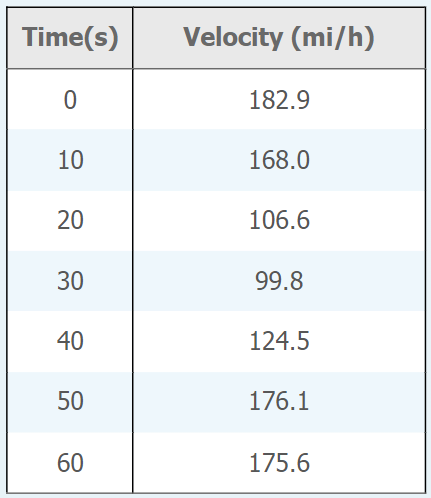
\includegraphics[scale=0.4]{img/img-0.png}
        \end{center}
        \begin{enumerate}
            \item Estimate the distance the race car traveled during this time period using the velocities at the beginning of the time intervals.\\
                The distance the race car traveled during this time period is:
                \[Distance = 182 \times 1/60 = 91/30 (miles)\]
            \item Give another estimate using the velocities at the end of the time periods.\\
                The distance the race car traveled during this time period is:
                \[Distance = 175.6 \times 1/60 = 439/150 (miles)\]
            \item Are your estimates in parts (a) and (b) upper and lower estimates? Explain.\\
                The average velocity is:
                \[\frac{182.9 + 168 + 106.6 + 99.8 + 124.5 + 176.1 + 175.6}{7} \approx 122.4 \]
                The estimates in parts (a) and (b) is upper estimates because both is larger than 122.4 mi/h. 
        \end{enumerate}
        \setcounter{enumi}{15}
        \item Use Definition 2 to find an expression for the area under the graph of $f$ as a limit. Do not evaluate the limit.
        \[f(x) = \frac{2x}{x^2+1} \text{, } 1 \leq x \leq 3\]
        \[\Delta x = \frac{3-1}{n} = \frac{2}{n}\]
        \[x_i = 1 + i\Delta x = 1 + \frac{2i}{n}\]
        \[Area = \lim_{n \to \infty} \Sigma^{n}_{i = 1}f(x_i)\Delta x = \lim_{n \to \infty} \Sigma^{n}_{i = 1}\frac{2(1 + \frac{2i}{n})}{(1 + \frac{2i}{n})^2+1}\times\frac{2}{n}\]
        \setcounter{enumi}{20}
        \item Determine a region whose area is equal to the given limit. Do not evaluate the limit.
        \[lim_{n\to\infty} \Sigma^{n}_{i=1} \frac{2}{n}\times \frac{1}{1+(2i/n)} = lim_{n\to\infty} \Sigma^{n}_{i=1} f(x_i) \Delta x\]
        \[f(x) = \frac{1}{x}\]
        \[\Delta x = \frac{2}{n}\]
        \[x_i = 1 + \frac{2i}{n}\]
        Hence, the region under the graph 
        \[f(x) = \frac{1}{x} \text{ with } 1 \leq x \leq 3\]
\end{enumerate}
\end{document}